% >>>>>>>>>>>>>>>>>>
\slide{Solução Proposta}{

\begin{itemize}
    \item Descrição do Ambiente
    \item Modelagem das Aeronaves
    \item Modelagem da Negociação como MDP
\end{itemize}
}

% >>>>>>>>>>>>>>>>>>
\slide{Descrição do Ambiente}{
\begin{figure}[]
    \centering
    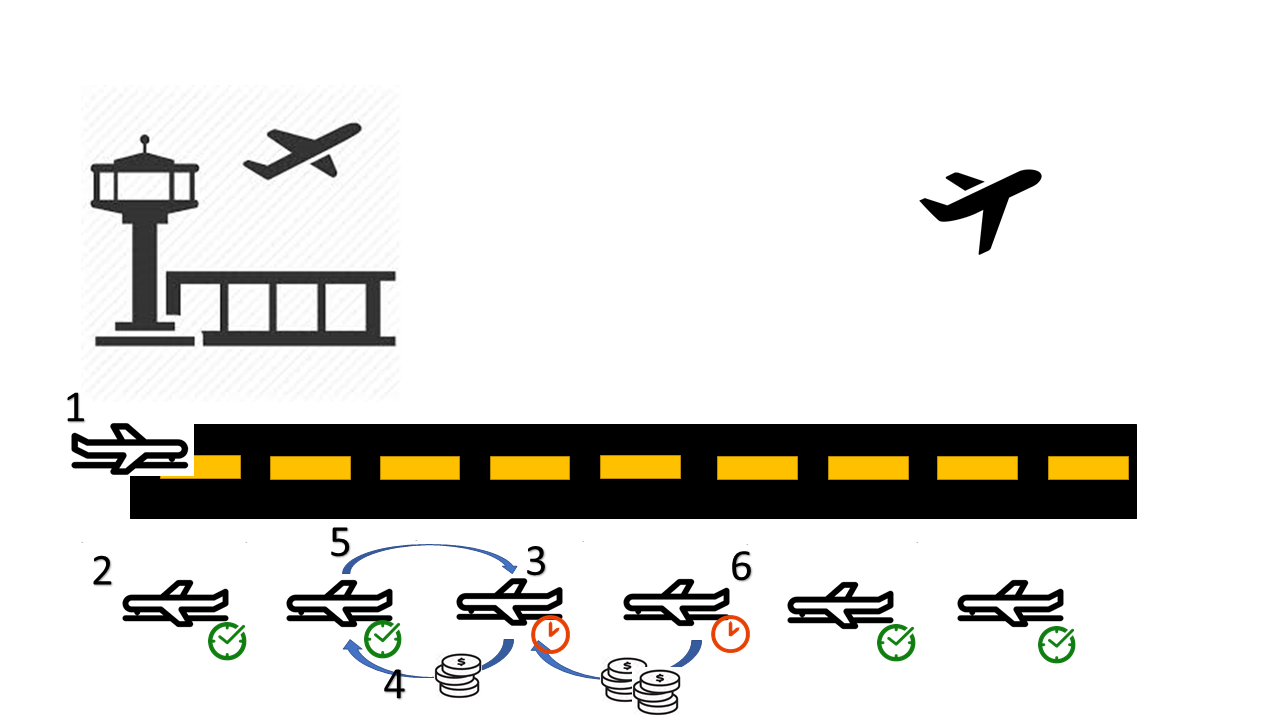
\includegraphics[scale=0.25]{img/cenario.png}
    %\caption{Modelo Geral da Negociação de Slots de Decolagem}
    \label{fig:cenario}
\end{figure}
}

\slide{Classes}{
\begin{figure}[]
    \centering
    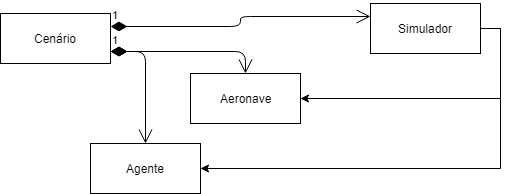
\includegraphics[scale=0.6]{img/class.png}
    %\caption{Plano de Voo Regular}
    \label{fig:PlanoVoo}
\end{figure}
}


\slide{Concepção da Oferta}{
 \begin{figure}[H]
    \centering
    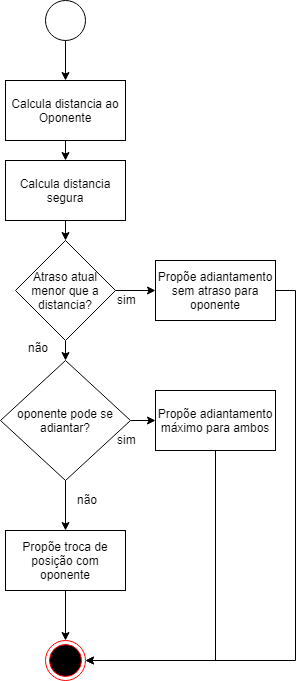
\includegraphics[scale=0.20]{img/melhor_oferta.png}
    \caption{Fluxograma de concepção da melhor oferta(pag-23)}
    \label{fig1:melhor_oferta}
    \end{figure}
}
\slide{Avaliação da Oferta}{
    \begin{figure}[H]
    \centering
    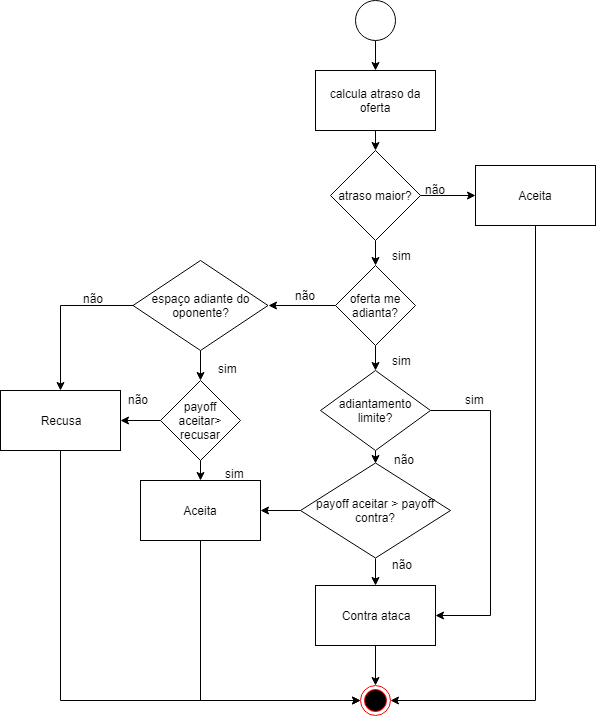
\includegraphics[scale=0.20]{img/avalia_oferta.png}
    \caption{Fluxograma de avaliação da oferta(pag-24)}
    \label{fig:avalia_oferta}
    \end{figure}
}

\slide{Contra Oferta}{
       
    \begin{figure}[H]
    \centering
    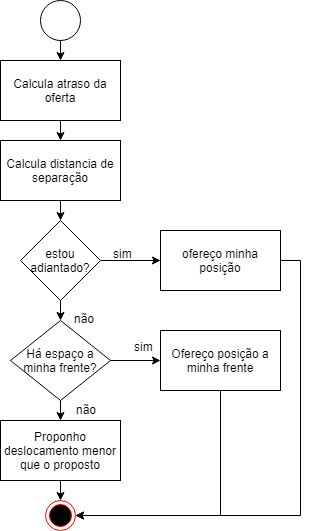
\includegraphics[scale=0.30]{img/contra_oferta.png}
    \caption{Fluxograma de concepção da contra-oferta(pag-25)}
    \label{fig:contra_oferta}
    \end{figure}

}
\slide{Árvore de Negociação}{
    \begin{figure}[H]
        \centering
        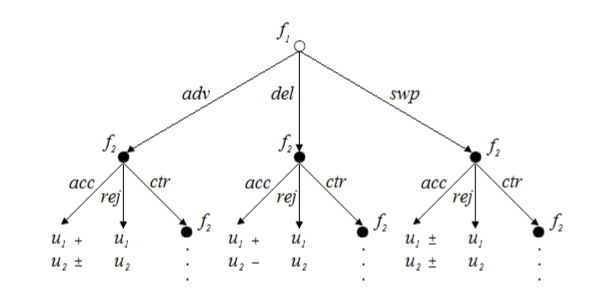
\includegraphics[scale=0.5]{img/arvore_negociacao.png}
        \caption{Árvore de Negociação entre duas Aeronaves}
        \label{fig:negociacao_aeronaves}
    \end{figure}}
    

\slide{Significância das Aeronaves}{
    A significância de uma aeronave é dada por:
    \begin{equation}
        \sigma = vt_{f}B+p
    \end{equation}
    Sendo $v$ a velocidade da aeronave, $t_{f}$ o tempo até o destino, $B$ o porte da aeronave e $p$ o número de passageiros.  
}

\slide{Custo das Aeronaves}{
    Desta forma, a significância de uma aeronave é dada por:
    \begin{equation}
        k=\dfrac{l\gamma}{D}\sigma
    \end{equation}
    Sendo: l o atraso atual da aeronave, D o atraso máximo aceito pela aeronave, $\gamma$ a importância da companhia aérea para o aeroporto e $\sigma$ a significância da Aeronave. 
}


    
    
\slide{Modelagem do Processo de Negociação como MDP}{
   
    \begin{itemize} 
        \item Estados são definido por: \textbf{atraso do agente}, \textbf{atributos do oponente}, \textbf{rodada}  e \textbf{papel}.
        \item Equilíbrio entre Especificidade e Generalidade.
    \end{itemize}
}


\slide{Ações Disponíveis}{
    \begin{itemize}
    \item Dependem do papel do agente na negociação. 
    \item Como proponente o agente pode escolher entre:
        \begin{itemize}
            \item adiantar-se: Adianta-se sem incutir atraso ao oponente. 
            \item avançar: Oponente se adianta o suficiente para que o agente melhore sua posição. 
            \item swap: Oponente troca de posição com o agente. 
        \end{itemize}
    \item Para cada ação, o agente pode ofertar 0\%, 25\% ou 50\% de seu ganho.
    \end{itemize}
}
\slide{Ações Disponíveis}{
    Como oponente o agente pode:
    \begin{itemize}
        \item Aceitar: oferta é efetivada e negociação acaba.
        \item Recusar: negociação acaba e árbitro escolhe oferta a ser efetivada.
        \item Contra-atacar: negociação continua, aeronaves trocam de papéis.
    \end{itemize}
    }    
\slide{Ações Disponíveis}{
    A ação de contra-atacar é expandida para as 4 contra-ofertas possíveis:
    \begin{itemize}
        \item realizar um atraso programado e ceder sua posição atual ao proponente
        \item oferecer o espaço adiante na fila se este estiver livre
        \item oferecer um espaço posterior
        \item adiantar-se
    \end{itemize}
}

\slide{Função de Transição}{
\begin{itemize}
    \item Depende apenas das ações realizadas pelas aeronaves e do estado no qual aeronave se encontra.
    \item As ações de aceitar e rejeitar encerrem a negociação com uma aeronave.
    \item Não levam necessariamente o agente a um estado terminal.
 
\end{itemize}
}
\slide{Função de Recompensa}{
\begin{itemize}
    \item Caso a oferta seja aceita, a recompensa dada ao agente é igual a diferença no custo do atraso entre a nova posição e a última.
    \item Caso o resultado seja a recusa, é dado uma recompensa negativa com valor constante. O mesmo ocorre no caso de contra-oferta. 
\end{itemize}
 }
